\section{TikZ/PGFplots + Animate 绘制动画}

\begin{lstlisting}[gobble=8]
           \documentclass{beamer}
           \usepackage{tikz, tkz-euclide}
           \usepackage{animate}
           \usetikzlibrary{math, calc}
           \begin{document}
           \begin{animateinline}[poster=31, controls={play,step,stop}]{24}
            \multiframe{361}{rtheta=0+1}
            {\begin{tikzpicture}[scale=1]
                    \path[use as bounding box] (-3.5,-2) rectangle (7.2,2;
                    \draw[rounded corners] (-3.5,-2) rectangle (7.2,2);
                    \tikzmath{function fCosseno(\x){return cos(\x);};
                        function degreeToRad(\d){ return {pi}*\d/180;};}
                    \draw[->,>=latex,thick] (-0.3,0) -- (7,0)node[below]{\(x\)};
                    \draw[->,>=latex,thick] (0,-1.5) -- (0,1.5)node[left]{\(y\)};
                    \draw[ultra thick, red, samples=50, domain=0:{2*pi}] plot (\x, {cos(\x r)});
                    \node at (0,0) [below left]{\(O\)};
                    \node at ({pi/2},0) [below]{\(\frac{\pi}{2}\)};
                    \node at ({pi},0) [below]{\(\pi\)};
                    \node at ({3*pi/2},0) [below]{\(\frac{3\pi}{2}\)};
                    \node at ({2*pi},0) [below]{\(2\pi\)};
                    \draw[thin, dashed] ({2*pi}, 0) -- ({2*pi},1);\draw (-2,0) circle (1cm);
                    \draw[->,>=latex,thick] (-3.5,0) -- (-0.5,0);
                    \draw[->,>=latex,thick] (-2,-1.5) -- (-2,1.5);
                    \coordinate (A) at (-2,0);\coordinate (B) at (-2,1);
                    \coordinate (C) at (-2,-1);\coordinate (D) at (-3,0);
                    \coordinate (E) at (-1,0);\coordinate (P) at ($(A) + (\rtheta:1)$);
                    \draw[thick] (A) -- (P);
                    \draw[thin, dashed, red] ($(D)!(P)!(E)$) -- (P) -- ($(B)!(P)!(C)$);
                    \draw[->, >=stealth] (-1.6,0) arc [start angle=0, end angle=\rtheta, radius=0.4];
                    \coordinate (Q) at ($(A) + ({fCosseno(\rtheta)},0)$);
                    \coordinate (R) at ($({-2+fCosseno(\rtheta)}, {fCosseno(\rtheta)})$);
                    \draw[ultra thick, red] (A) -- (Q) -- (R);
                    \tkzDrawArc[thin, red](Q,R)(A)
                    \draw[thin, red, dashed] (R) -- ({degreeToRad(\rtheta)}, {fCosseno(\rtheta)}) -- ({degreeToRad(\rtheta)},0);
                    \draw[fill=black] ({degreeToRad(\rtheta)}, {fCosseno(\rtheta)}) circle (1pt);
                \end{tikzpicture}}
         \end{animateinline}
        \end{document}
\end{lstlisting}

        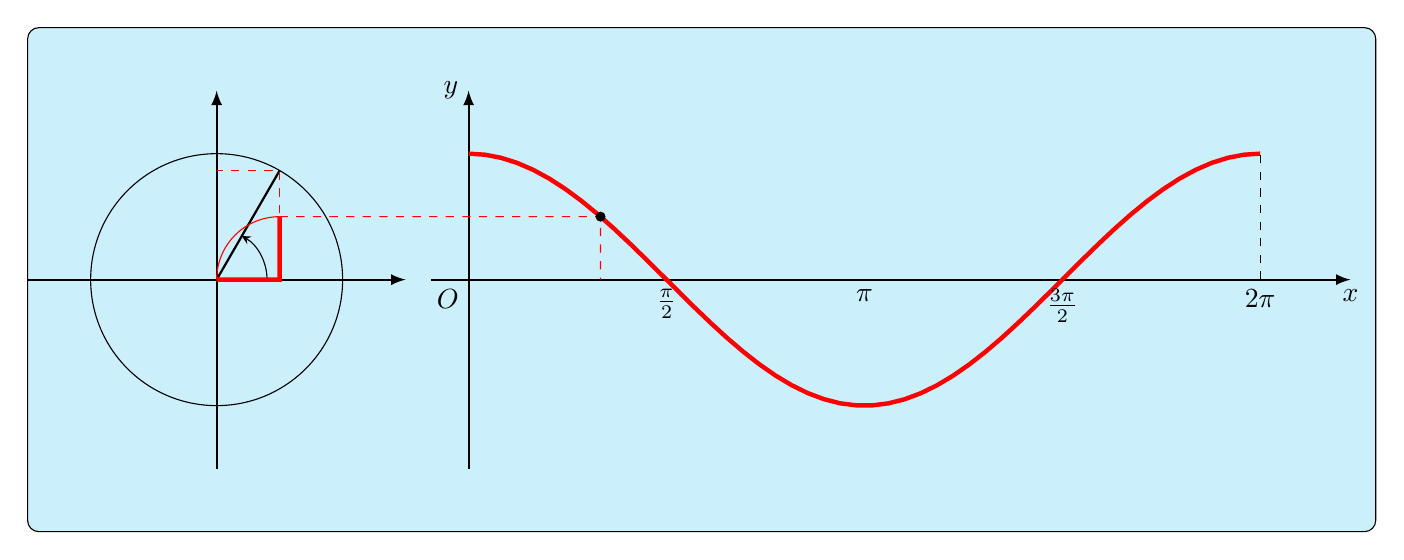
\begin{tikzpicture}[scale=1.6]
            \path[use as bounding box] (-3.5,-2) rectangle (7.2,2);
            \draw[rounded corners,fill=cyan!20!white] (-3.5,-2) rectangle (7.2,2);

            \tikzmath{
                function fCosseno(\x){
                    return cos(\x);
                };
                function degreeToRad(\d){
                    return {pi}*\d/180;
                };
            }
            \draw[->,>=latex,thick] (-0.3,0) -- (7,0)node[below]{\(x\)};
            \draw[->,>=latex,thick] (0,-1.5) -- (0,1.5)node[left]{\(y\)};
            \draw[ultra thick, red, samples=50, domain=0:{2*pi}]
            plot (\x, {cos(\x r)});
            \node at (0,0) [below left]{\(O\)};
            \node at ({pi/2},0) [below]{\(\frac{\pi}{2}\)};
            \node at ({pi},0) [below]{\(\pi\)};
            \node at ({3*pi/2},0) [below]{\(\frac{3\pi}{2}\)};
            \node at ({2*pi},0) [below]{\(2\pi\)};
            \draw[thin, dashed] ({2*pi}, 0) -- ({2*pi},1);
            \draw (-2,0) circle (1cm);
            \draw[->,>=latex,thick] (-3.5,0) -- (-0.5,0);
            \draw[->,>=latex,thick] (-2,-1.5) -- (-2,1.5);
            \coordinate (A) at (-2,0);
            \coordinate (B) at (-2,1);
            \coordinate (C) at (-2,-1);
            \coordinate (D) at (-3,0);
            \coordinate (E) at (-1,0);
            \coordinate (P) at ($(A) + ( 60:1)$);
            \draw[thick] (A) -- (P);
            \draw[thin, dashed, red] ($(D)!(P)!(E)$) -- (P) -- ($(B)!(P)!(C)$);
            \draw[->, >=stealth] (-1.6,0) arc [start angle=0, end angle= 60, radius=0.4];
            \coordinate (Q) at ($(A) + ({fCosseno( 60)},0)$);
            \coordinate (R) at ($({-2+fCosseno( 60)}, {fCosseno( 60)})$);
            \draw[ultra thick, red] (A) -- (Q) -- (R);
            \tkzDrawArc[thin, red](Q,R)(A)
            \draw[thin, red, dashed] (R) -- ({degreeToRad( 60)}, {fCosseno( 60)}) -- ({degreeToRad( 60)},0);
            \draw[fill=black] ({degreeToRad( 60)}, {fCosseno( 60)}) circle (1pt);
        \end{tikzpicture}
 